\setAuthor{}
\setRound{lõppvoor}
\setYear{2019}
\setNumber{G 3}
\setDifficulty{3}
\setTopic{TODO}

\prob{Lennuk}
\begin{wrapfigure}[12]{r}{0.37\textwidth}
  \vspace{-28pt}
  \begin{center}
  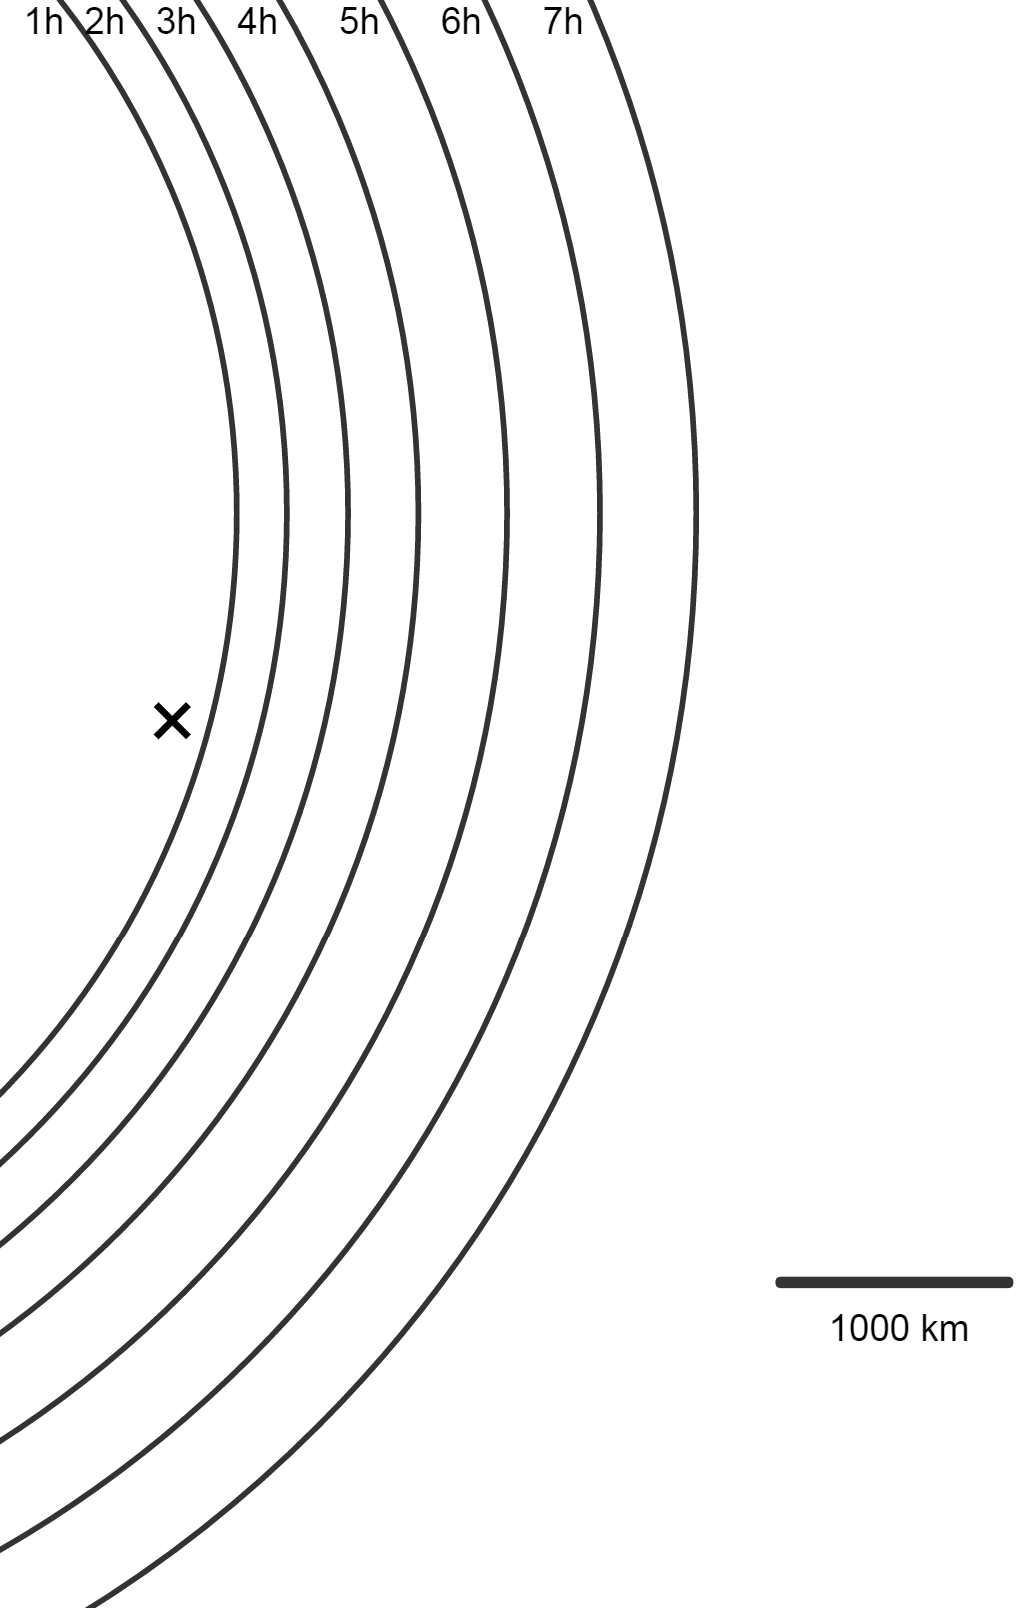
\includegraphics[scale=0.2]{2019-v3g-03-yl.png}
  \end{center}
  \vspace{-20pt}
\end{wrapfigure}


Joonisel on lennuki algne asukoht märgitud ristiga. Iga tunni järel mõõdeti lennuki kaugust fikseeritud punktist. Saadud kaugused on joonisel märgitud ringjoonena mõõtepunkti ümber. Konstrueerige kõikvõimalikud lennuki trajektoorid $\SI{7}{h}$ jooksul, kui on teada, et pärast starti lendas lennuk $\SI{4}{h}$ otse, muutis seejärel suunda ning lendas ülejäänud aja samuti otse. Eeldada, et lennuki kiirus maapinna suhtes oli ühtlaselt $\SI{500}{km/h}$. Lahendus esitada lisalehel.
\textit{Märkus.} Suuna muutus võis olla ka väga väike. 


\hint

\solu
\begin{wrapfigure}{r}{0.41\textwidth}
  \vspace{-15pt}
  \begin{center}
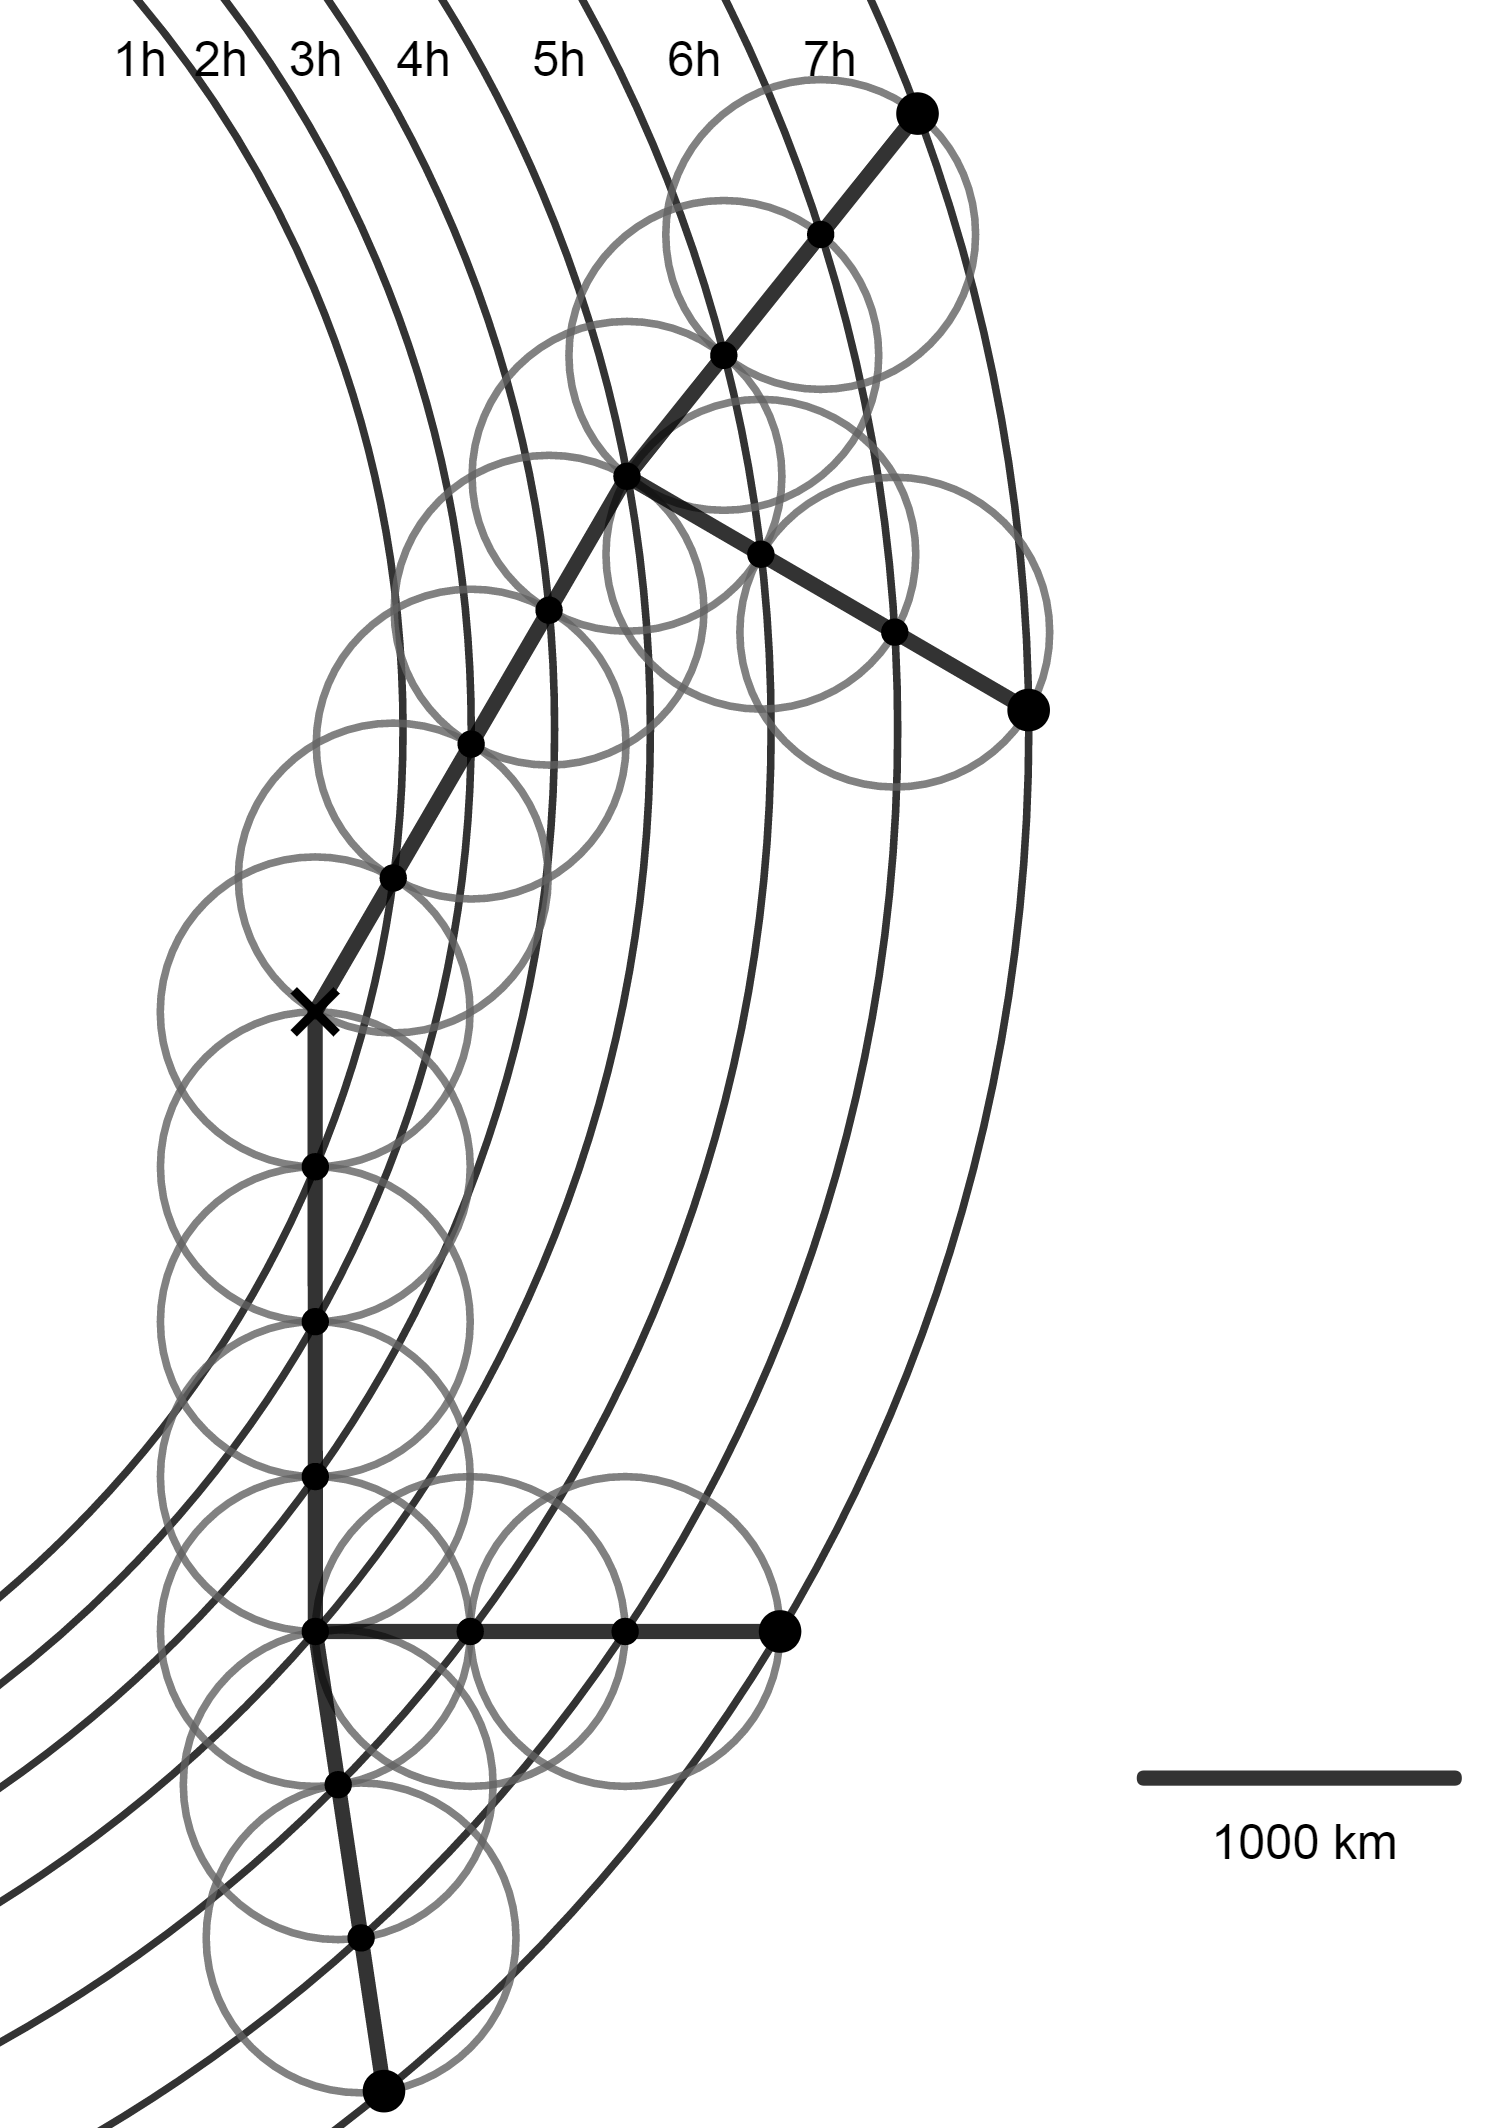
\includegraphics[scale=0.15]{2019-v3g-03-sol.png}
    % Pildi allikas Wikimedia Commons https://upload.wikimedia.org/wikipedia/commons/4/4f/Curling_stones.jpg
  \end{center}
  \vspace{-20pt}
\end{wrapfigure}

Teame, et suured ringjooned märgivad lennuki asukohta iga tunni järel ning ühe tunniga läbib lennuk $\SI{500}{km}$. Joonisel oleva mõõtkava järgi saame $\SI{500}{km}$ vastava pikkuse joonisel. Võtame selle pikkuse ja joonestame sirkliga vastava raadiusega ringjoone lennuki algasukoha ümber. See ringjoon märgib lennuki asukohta $1h$ pärast õhkutõsu ning selle lõikepunktid olemasoleva esimese suure ringjoonega (mis märgib samuti lennuki asukohta $\SI{1}{h}$ pärast õhkutõsu) annavad meile lennuki võimalikud asukohad $\SI{1}{h}$ pärast. Kuna me ei tea, millises suunas lennuk lendas, peame lennuki teekonda mõlemast punktist edasi konstrueerima, joonestades uute punktide ümber samuti $\SI{500}{km}$ vastava ringjoone. Kuna aga teame, et lennuk lendas $\SI{4}{h}$ järjest otse, saame hakata lõikepunkte välistama, sest sobivad punktid moodustavad sirge. $\SI{4}{h}$ vastava ringjoone juures teame vaid seda, et lennuk muutis suunda. Seega saame kummagi algse teekonna kohta veel 2 võimalikku uut suunda (kokku 4 võimalikku suunda). Teades, et lennuk lendas edaspidi samuti vaid otse, saame kõik 4 teekonda lõpuni konstrueerida.
\probend